\documentclass[12pt]{article}
\usepackage{float}
\usepackage{amsmath}
\usepackage{graphicx}
\usepackage{hyperref}
\usepackage{listings}
\usepackage{color}
\usepackage{booktabs}

\definecolor{codebg}{rgb}{0.95,0.95,0.95}
\definecolor{codeframe}{rgb}{0.8,0.8,0.8}

\lstset{
    backgroundcolor=\color{codebg},
    frame=single,
    frameround=tttt,
    rulecolor=\color{codeframe},
    basicstyle=\ttfamily,
    columns=fullflexible,
    breaklines=true
}

\title{Analiza statystyczna przyznawania funduszy UE gminom}
\author{Krzysztof Rudnicki, Michał Sar}
\date{\today}

\begin{document}

\maketitle

\tableofcontents

\begin{abstract}
    This is a brief summary of our study, its results, and major conclusions.
\end{abstract}

\section{Wstęp}
\paragraph{Kontekst}
W 2024 roku mija 20 lat od wstąpienia Polski do Unii Europejskiej \cite{1}. 
Od tamtej pory bilans Polski w stosunku do Brukseli wynosi 175 miliardów euro na plus dla Polski \cite{2}. W samym 2023 roku Polska otrzymała z UE prawie 3.5 miliarda złotych, wpłacając niecały miliard złotych \cite{3}. W naszej pracy ponawiamy analizę statystyczną wykonaną sprzed 7 lat, na nowych danych, od początku roku 2014 do końca roku 2023.
\paragraph{Cel}
Celem pracy jest sprawdzenie, jakie dane na temat gminy najbardziej korelują z liczbą przyznanych funduszy Unii Europejskiej danej gminie.
\paragraph{Hipoteza}
Gęstość zaludnienia jest \textbf{najważniejszym} czynnikiem wpływającym na przyznanie środków unijnych.
\paragraph{Metoda badawcza}
\begin{enumerate}
    \item Zebrać dane UE.
    \item Zebrać dane gmin.
    \item Połączyć dane po numerze TERYT.
    \item Przeanalizować dane.
    \item Wyświetlić wyniki.
\end{enumerate}

\section{Omówienie rozdziałów}
Na początku artykułu przedstawiamy, dlaczego wybraliśmy taki temat, co chcemy osiągnąć naszą pracą, w jaki sposób chcemy to osiągnąć i jaki rezultat ostatecznie udało nam się pokazać. 
Następnie opisujemy istniejącą literaturę na temat środków unijnych, z którą się zapoznaliśmy, i przedstawiamy, w czym różni się nasza praca od istniejących. 
Potem tłumaczymy nasz proces badawczy, w jaki sposób zbieraliśmy i łączyliśmy dane, jak je analizowaliśmy i jak przedstawialiśmy wyniki. 
Kontynuując, pokazujemy, co otrzymaliśmy ostatecznie w wyniku naszej pracy. 
Przedostatni rozdział zajmuje się dyskusją wyników; przedstawiamy, co udało nam się osiągnąć i dlaczego, czego nie udało nam się osiągnąć i dlaczego oraz przede wszystkim konfrontujemy wynik z naszą hipotezą. 
Na końcu podsumowujemy całą pracę i przedstawiamy spis literatury, z której korzystaliśmy.

\section{Opis literatury}
\paragraph{Decision trees: from efficient prediction to responsible AI}
Artykuł poświęcony jest omówieniu drzew decyzyjnych, rozpoczyna od zdefiniowania, czym drzewo decyzyjne jest, jakie są jego unikalne cechy, gdzie jest stosowane, jakie ma wady i potencjalne zagrożenia oraz jak można je zminimalizować \cite{4}. 
Wybraliśmy ten artykuł, gdyż opisuje jedną z głównych metod, którą zamierzamy stosować w naszym procesie badawczym do przeanalizowania danych.
\paragraph{Application of Successful EU Funds Absorption Models to Sustainable Regional Development}
Artykuł wykorzystał ankiety, pytając 244 osób o to, jak efektywnie wykorzystywane były fundusze UE w Polsce, Słowenii, Węgrzech i Chorwacji. Artykuł podkreśla znaczenie możliwości technicznych, administracyjnych, koordynacji pomiędzy instytucjami i dobrymi mechanizmami nadzorowania funduszy europejskich jako kluczowe dla skutecznego wykorzystywania funduszy unijnych \cite{5}. 
Artykuł przydał się nam w ocenie, jakie parametry pozytywnie wpływają na korzystanie z funduszy UE i jakie moglibyśmy śledzić w naszym modelu. W naszym artykule zamiast ankiet wykorzystujemy dostępne już dane, a wyniki staramy się stworzyć przy użyciu modeli statystycznych. Dodatkowo zajmujemy się przedstawieniem, jakie parametry wpływają na przyznanie środków UE, a nie na to, w jaki sposób można te środki skutecznie wykorzystywać.
\paragraph{It’s not about the money. EU funds, local opportunities, and Euroscepticism}
Artykuł opisuje, jak pieniądze z Unii Europejskiej wpływają na eurosceptycyzm w danym kraju na podstawie Walii w kontekście referendum "Brexit". 
Badanie wykorzystuje metodę Regression Discontinuity Design (RDD), wybrano Walię z uwagi na różnicę w ilości pieniędzy przekazanych poszczególnym rejonom. 
Autorzy wykazali, że sama ilość pieniędzy przekazana danemu regionowi nie zwiększa znacznie poparcia dla Unii Europejskiej, natomiast duże nakłady powiązane z widoczną, namacalną poprawą na lokalnym rynku wpływają pozytywnie na postrzeganie Unii Europejskiej w lokalnych społecznościach \cite{6}. 
Nasz artykuł koncentruje się na tym, co wpływa na przyznanie funduszy unijnych, a nie na samą reakcję na ich przyznanie.

\section{Proces badawczy}
Proces badawczy podzieliliśmy na trzy zasadnicze etapy: zebranie danych, przeanalizowanie ich i zaprezentowanie wyników.

\paragraph{Zbieranie danych}
Wszystkie dane pobieraliśmy ze strony GUS-u:
\href{https://bdl.stat.gov.pl/bdl/start}{https://bdl.stat.gov.pl/bdl/start} 
Dane wybieraliśmy z zakładki "Popularne podgrupy", następnie wybieraliśmy wszystkie lata, które nas interesowały (od 2014 do 2023 roku włącznie), po przejściu dalej wybieraliśmy wszystkie gminy, finalnie otrzymując tablicę, którą pobieraliśmy do formatu CSV.
\begin{figure}[H]
    \caption{Strona GUS z zaznaczonymi popularnymi podgrupami}
    \centering
    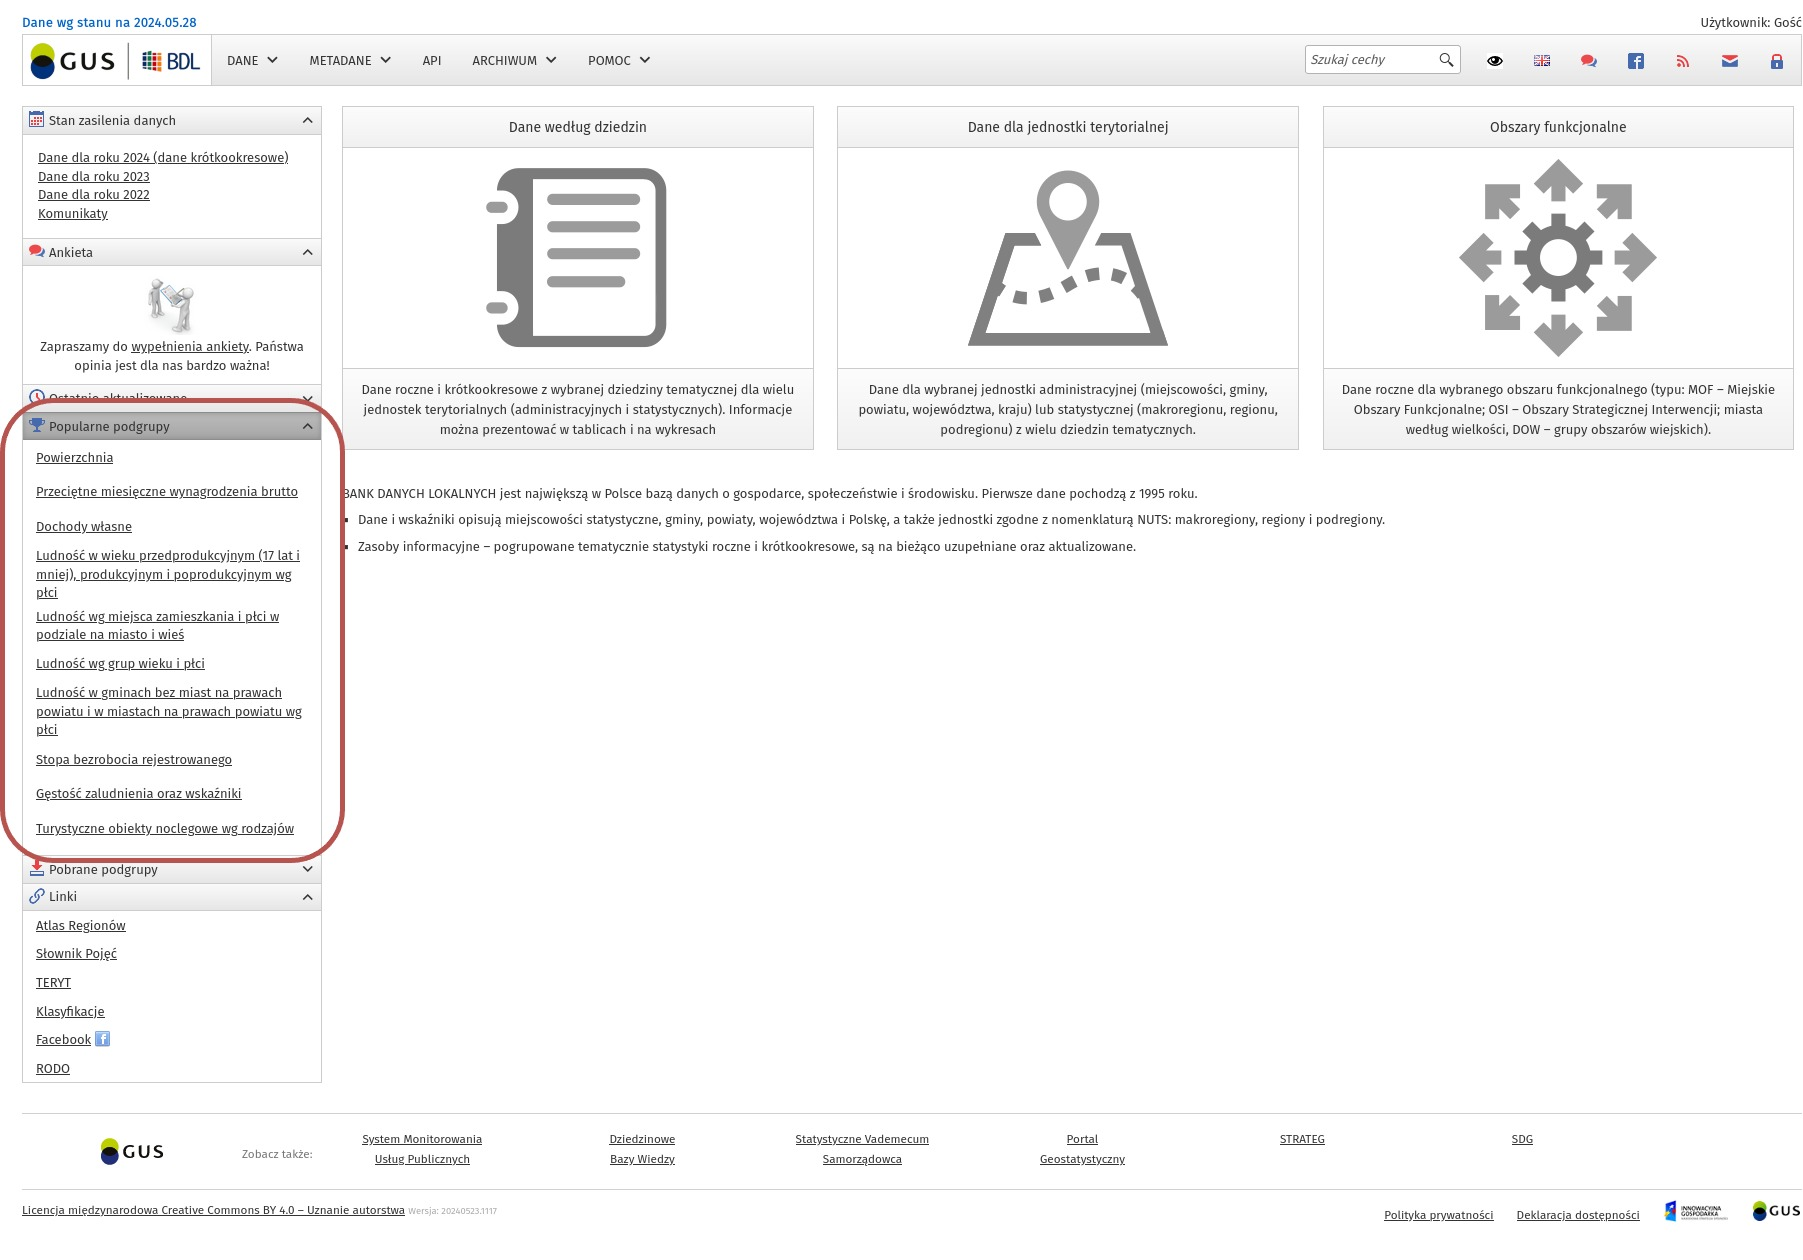
\includegraphics[width=1.0\textwidth]{gus}
\end{figure}
\begin{figure}[H]
    \caption{Strona GUS z zaznaczonymi latami i powierzchnią}
    \centering
    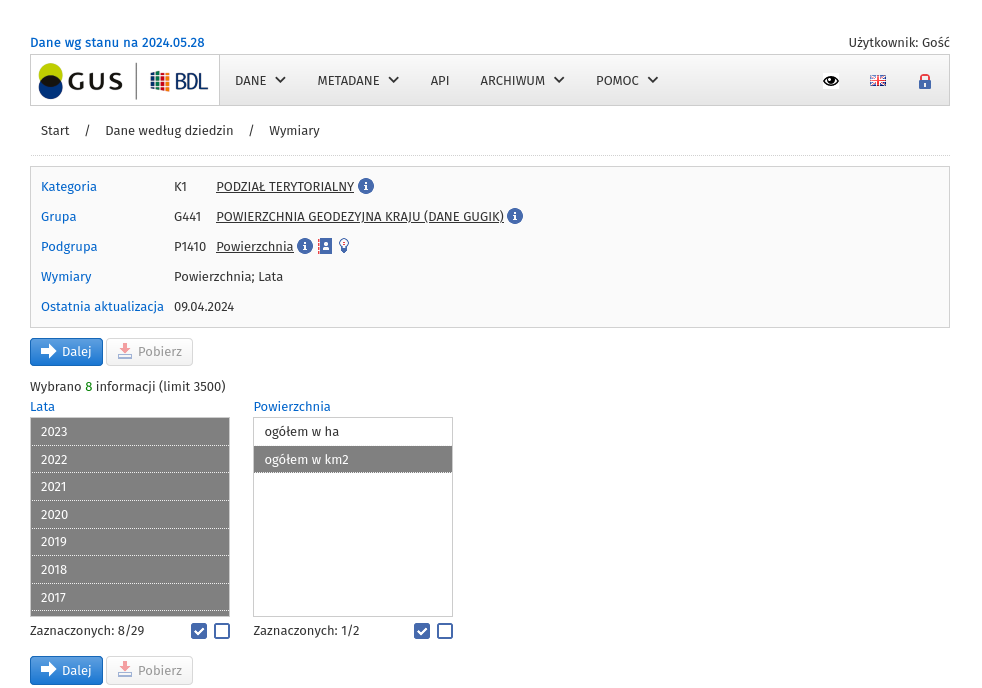
\includegraphics[width=1.0\textwidth]{dane3}
\end{figure}
\begin{figure}[H]
    \caption{Strona GUS z zaznaczonymi powiatami}
    \centering
    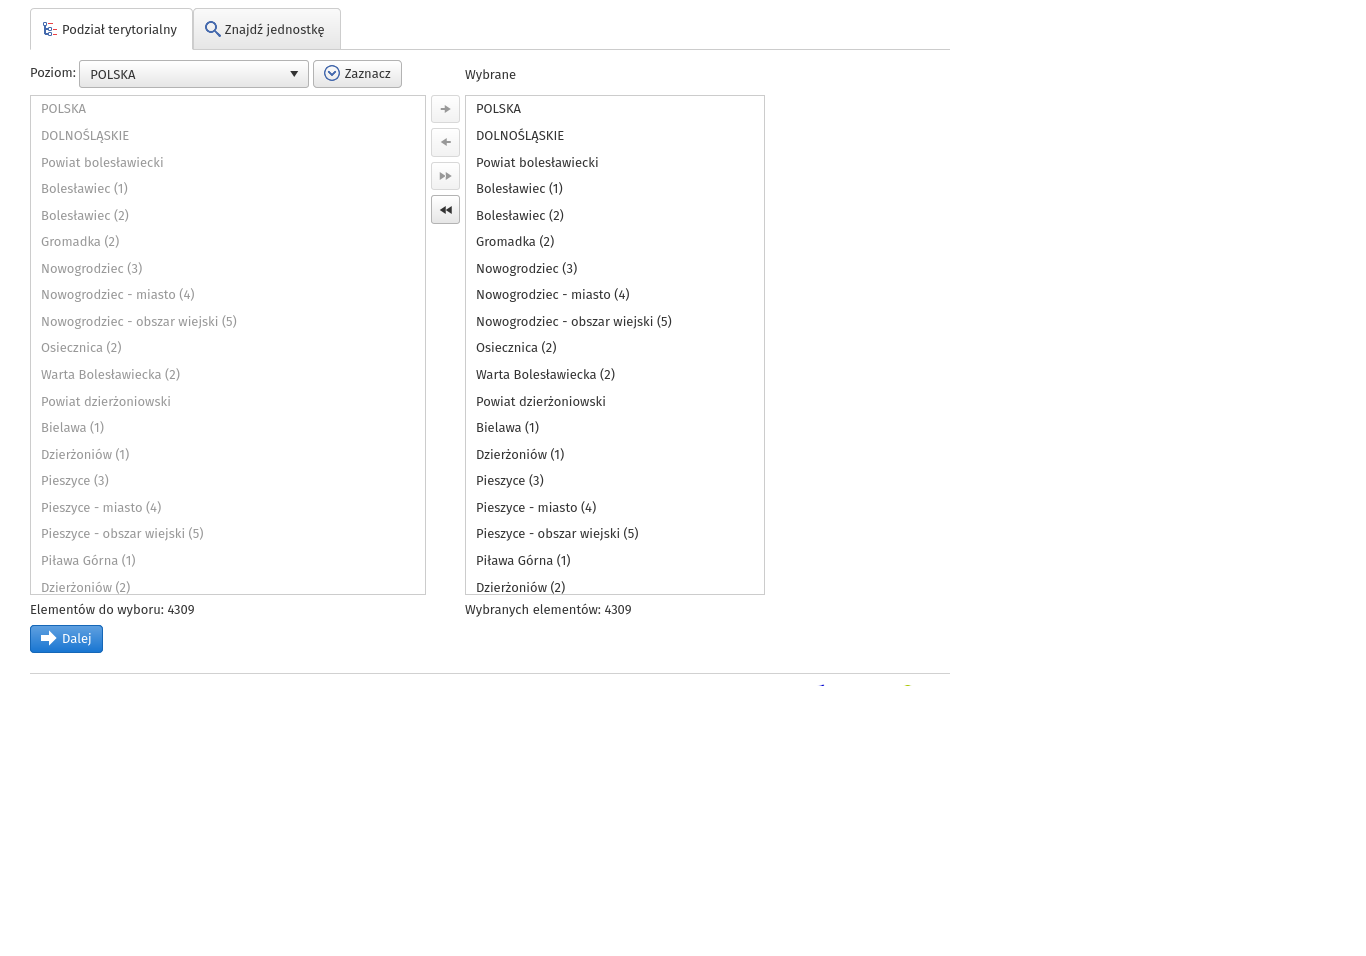
\includegraphics[width=1.0\textwidth]{dane4}
\end{figure}
\begin{figure}[H]
    \caption{Dane o powierzchni z możliwością eksportu do CSV}
    \centering
    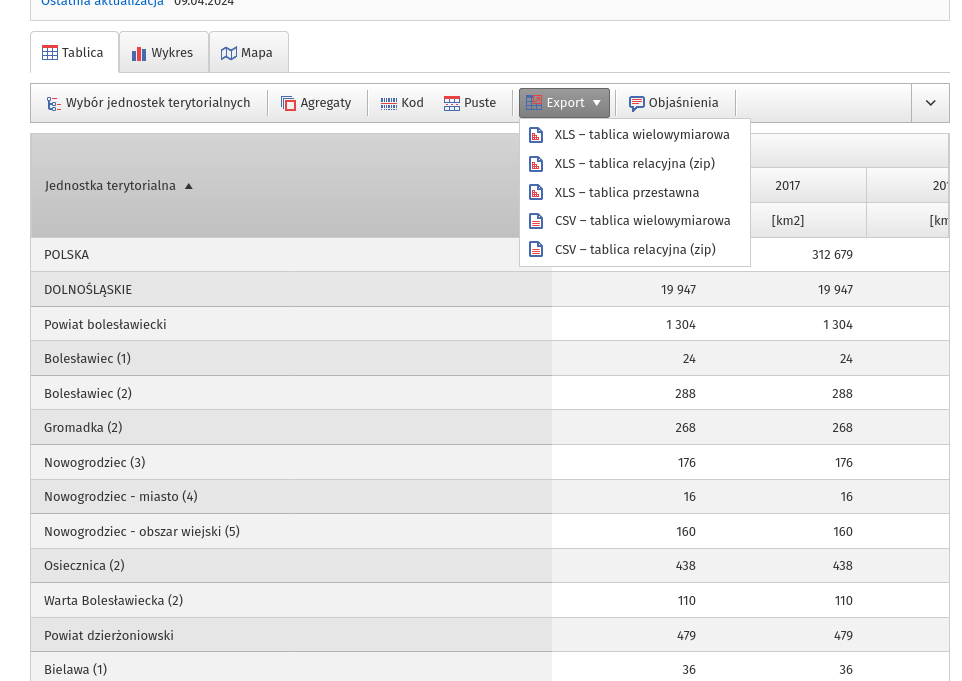
\includegraphics[width=1.0\textwidth]{dane5}
\end{figure}

\paragraph{Przygotowywanie danych}
Dane musieliśmy przeprocesować przed ich wykorzystaniem, usuwaliśmy wiersze:
\begin{itemize}
    \item Zawierające niepełny numer TERYT.
    \item Zawierające wartości Null albo puste.
\end{itemize}
Wybraliśmy w sumie 100 parametrów, na podstawie których ocenialiśmy wpływ na dotacje z UE. Można je podzielić na grupy:
\begin{enumerate}
    \item Finansowe (dochody, wpływy, podatki).
    \item Ludność (całkowita, na płeć, wiek przedprodukcyjny/produkcyjny/poprodukcyjny, gęstość zaludnienia).
    \item Województwo.
    \item Wymeldowania i zameldowania.
    \item Turystyka.
    \item Bezrobocie.
    \item Typ gminy.
    \item Odległość od Warszawy lub centrum decyzyjnego.
\end{enumerate}
Dzieliliśmy dane o dofinansowaniu UE na podstawie programów:
\begin{itemize}
    \item Program Operacyjny Infrastruktura i Środowisko 2014-2020.
    \item Program Operacyjny Inteligentny Rozwój.
    \item Program Operacyjny Polska Cyfrowa.
    \item Program Operacyjny Wiedza Edukacja Rozwój.
    \item Program Operacyjny Polska Wschodnia.
\end{itemize}

\paragraph{Analiza danych}
Wykorzystaliśmy model drzew decyzyjnych regresyjnych, wykorzystujących "Recursive Feature Elimination" (RFE). 
Trenowaliśmy model na głębokościach od 3 do 28 i na liczbie cech od 2 do 20. 
W ten sposób szukaliśmy najlepszego modelu, takiego, który wykazywał najmniejszy błąd MSE. 
Najlepsze parametry uzyskaliśmy dla głębokości 20 i liczby cech 13.
\begin{lstlisting}
    max_depth: 20, n_features: 13, mse_train: 89643306022.6, mse_test: 879912454221.0 <-
\end{lstlisting}

\paragraph{Przedstawienie wyników}
Wyniki przedstawiliśmy na wykresach, wykorzystując pythonową bibliotekę matplotlib.

\section{Wyniki}
\begin{figure}[H]
\caption{Błąd dla danych treningowych jako funkcja głębokości i liczby cech}
\centering
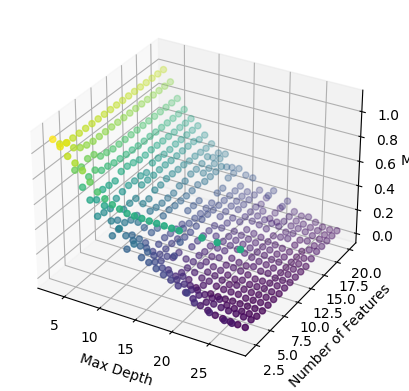
\includegraphics[width=1.0\textwidth]{output.png}
\end{figure}
\begin{figure}[H]
\caption{Błąd dla danych testowych jako funkcja głębokości i liczby cech}
\centering
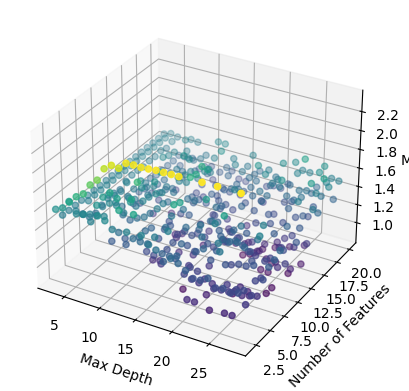
\includegraphics[width=1.0\textwidth]{output2.png}
\end{figure}
\begin{figure}[H]
\caption{Funkcja predykcji modelu co do wielkości finansowania porównana do prawdziwego finansowania, czerwieńsze kolory odpowiadają większej gęstości zaludnienia}
\centering
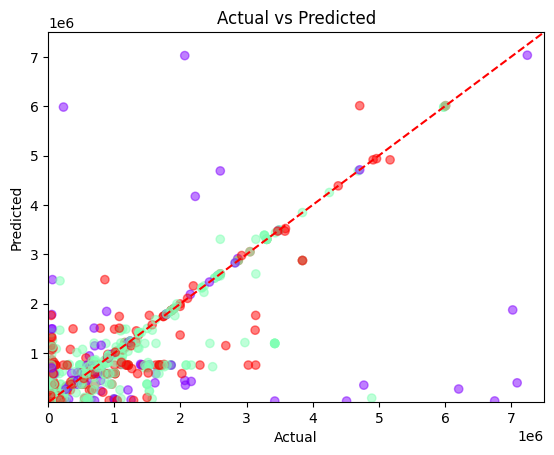
\includegraphics[width=1.0\textwidth]{output3.png}
\end{figure}
Parametry poniżej miały największy związek z wysokością wpływów z Unii Europejskiej do gminy.

\begin{table}[H]
    \centering
    \begin{tabular}{lr}
    \toprule
    \textbf{Kategoria} & \textbf{Wartość} \\
    \midrule
    Dochody z podatku od nieruchomości & 0.3853 \\
    Dochody z podatku od środków transportowych & 0.2161 \\
    Powierzchnia & 0.0911 \\
    Wynagrodzenie ogółem & 0.0670 \\
    Dochody z podatku PCC & 0.0581 \\
    Dochody razem & 0.0424 \\
    Dochody z majątku & 0.0292 \\
    Dochody z podatku od spadków & 0.0286 \\
    Dochody z podatku rolnego & 0.0277 \\
    Dochody z podatku od działalności gospodarczej & 0.0225 \\
    Wynagrodzenie w relacji do średniej & 0.0156 \\
    Dochody z podatku odrębne ustawy & 0.0107 \\
    Dochody z podatku leśnego & 0.0057 \\
    \bottomrule
    \end{tabular}
    \caption{Najistotniejsze dane gminy wpływające na przyznanie funduszy UE}
\end{table}

\section{Dyskusja}
\paragraph{Sukcesy}
Udało nam się zebrać dane z GUS-u i połączyć je z danymi o inwestycjach Unii Europejskich. Stworzyliśmy model, który na podstawie przygotowanych przez nas danych spróbował wykazać, jakie parametry gminy najbardziej wpływały na przyznanie środków unijnych.
\paragraph{Weryfikacja hipotezy}
Nasza hipoteza zgodnie z wynikami, które uzyskaliśmy, okazała się \textbf{fałszywa}. Nasz model za najważniejszą daną o gminie wpływającą na przyznanie środków z Unii Europejskiej uznał \textbf{dochód z podatków od nieruchomości}, a nie gęstość zaludnienia.
\paragraph{Niskie wartości korelacji}
Niestety wartości powiązania danych o gminie i wpływów z UE w naszym modelu mają niskie wartości, najwyższe rzędu 0.4, po czym drastycznie spadają do poziomu 0.01, 0.005.
\paragraph{Brak możliwości predykcji}
Nasz model \textbf{nie nadaje się} do wykorzystania w celu przewidywania wpływów inwestycji z UE do gminy w przyszłości. Wynika to z dynamicznie zmieniającej się sytuacji geopolitycznej. W ostatnich latach zdecydowany wpływ na działania Unii Europejskiej miały takie wydarzenia jak pandemia COVID-19 lub wojna w Ukrainie. Niemożliwe do przewidzenia wydarzenia na arenie międzynarodowej sprawiają, że predykcja przyszłych zachowań tak dużych instytucji jak Unia Europejska jest dla naszego modelu zadaniem nieosiągalnym.

\section{Konkluzja}
Analiza obaliła naszą hipotezę, że gęstość zaludnienia odgrywa największą rolę i zamiast tego wskazuje na dochód z podatków od nieruchomości. Nasz model, mimo że zidentyfikował pewne zależności, charakteryzuje się niskimi wartościami korelacji i ograniczoną zdolnością do przewidywania przyszłych funduszy.

Aby poprawić dokładność przyszłych analiz, sugerujemy wykorzystanie innych technik modelowania (gradient boosting, sieci neuronowe) oraz dodatkowych zmiennych, takich jak zmiany polityczne, ekonomiczne i społeczne. Rozważenie tych dynamicznych czynników może lepiej odzwierciedlić skomplikowane procesy decyzyjne w Unii Europejskiej i zwiększyć trafność prognozowania przyznawania funduszy.

\bibliographystyle{plain} % or any other style you prefer
\bibliography{references} % 'references' should be the name of your .bib file without the extension

\end{document}
